\documentclass[12pt,a4paper]{article}
\usepackage[polish]{babel}
\usepackage[T1]{fontenc}
\usepackage{lmodern}
\usepackage[utf8x]{inputenc}
\usepackage{hyperref}
\usepackage{url}
\usepackage{graphicx}
\usepackage{listings}
%\usepackage{xcolor}
\usepackage{color}
\usepackage{float}
\usepackage{multicol}
\usepackage{tikz-er2}
\usetikzlibrary{er,positioning,shadows}
\usepackage{makecell}
\renewcommand{\arraystretch}{1.5}

% TIKZ 
\tikzstyle{every entity} = [top color=white, bottom color=blue!30, 
                            draw=blue!50!black!100, drop shadow]
\tikzstyle{every weak entity} = [drop shadow={shadow xshift=.7ex, 
                                 shadow yshift=-.7ex}]
\tikzstyle{every attribute} = [top color=white, bottom color=yellow!20, 
                               draw=yellow, node distance=1cm, drop shadow]
\tikzstyle{every relationship} = [top color=white, bottom color=red!20, 
                                  draw=red!50!black!100, drop shadow]
\tikzstyle{every isa} = [top color=white, bottom color=green!20, 
                         draw=green!50!black!100, drop shadow]
                         
% LISTINGS
\definecolor{bluekeywords}{rgb}{0,0,1}
\definecolor{greencomments}{rgb}{0,0.5,0}
\definecolor{redstrings}{rgb}{0.64,0.08,0.08}
\definecolor{xmlcomments}{rgb}{0.5,0.5,0.5}
\definecolor{types}{rgb}{0.17,0.57,0.68}
\usepackage{listings}
\lstset{language=SQL,
captionpos=b,
frame=lines,
showspaces=false,
showtabs=false,
breaklines=true,
showstringspaces=false,
breakatwhitespace=true,
escapeinside={(*@}{@*)},
commentstyle=\color{greencomments},
keywordstyle=\color{bluekeywords},
stringstyle=\color{redstrings},
basicstyle=\ttfamily\small,
tabsize=4,
}                     

% SETTINGS
\addtolength{\hoffset}{-1.5cm}
\addtolength{\marginparwidth}{-1.5cm}
\addtolength{\textwidth}{3cm}
\addtolength{\voffset}{-1cm}
\addtolength{\textheight}{2.5cm}
\setlength{\topmargin}{0cm}
\setlength{\headheight}{0cm}
% GO GO GO
\title{Academic Data Deliverer\\Bazy Danych}
\author{Artur Bednarczyk, Dawid Grajewski, Damian Kwaśniok\\Politechnika Śląska\\Wydział Matematyki Stosowanej\\Informatyka, semestr IV}
\date{\today}

\begin{document}
	\maketitle
	\begin{figure}[H]
		\centering
		\includegraphics[width=0.5\linewidth]{LOGO2}
		\label{fig:logo}
	\end{figure}
	\clearpage
	\tableofcontents
	\clearpage
	\section{Opis projektu}
		\subsection{Opis}
			Aplikacja dla studentów umożliwiająca szybki i łatwy podgląd dostępnych materiałów! Każdy student może wybrać kierunki studiów, którymi jest zainteresowany i oglądać przypisane do nich notatki! W każdej chwili  może dodać nowe lub usunąć nieinteresujące go kierunki ze swojej listy. Aplikacja jest prosta w użytkowaniu, jednak wymaga połączenia z internetem.
		\subsection{Funkcjonalności}
			\subsubsection{Logowanie i Rejestracja}
				Załóż swoje konto, a będziesz mógł korzystać z aplikacji z każdego urządzenia, na którym jest zainstalowana i posiada dostęp do internetu! Zachowaj Twoje listy kierunków na swoim koncie!
			\subsubsection{Przypasanie do grup}
				Wybierz kierunki, które Cię interesują i przeglądaj materiały z nimi powiązane. W każdej chwili możesz dopisać do swojej listy nowe kierunki lub usunąć już niepotrzebne.
			\subsubsection{Notatki}
				Przeglądaj dostępne materiały z listy kierunków, którą sam utworzyłeś. Jeśli chcesz mieć dostęp offline to pobierz materiał w formie pliku!
	\section{Technologie}
			\subsection{Oprogramowanie}
			\begin{itemize}
			\item Visual Studio 2015 - Środowisko programistyczne.
			\item SourceTree - Kontrola wersji.
			\item GitHub - Repozytorium do przechowywania wersji online.
			\item Heroku - Chmura, w której przechowywana jest baza danych.
			\end{itemize}
			\subsection{Technologie}
			\begin{itemize}
			\item C\#
			\item .NET
			\item MySQL
			\end{itemize}
	\section{Baza Danych}
		\subsection{Diagram Encji}
		\scalebox{.65}{
			\begin{tikzpicture}[node distance=1.5cm, every edge/.style={link}]
				\node[entity] (users) {USERS};
					\node[attribute] (users_name) [above left = of users] {First Name} edge (users);
					\node[attribute] (users_last_name) [above = of users] {Last Name} edge (users);
					\node[attribute] (users_phone_number) [above right = of users] {Phone Number} edge (users);
					\node[attribute] (users_account_type) [left = of users] {Account Type} edge (users);
					\node[attribute] (users_mail) [below left = of users] {Mail} edge (users);
					\node[attribute] (users_login) [below = of users] {Login} edge (users);
					\node[attribute] (users_password) [below right = of users] {Password} edge (users);
				\node[relationship] (users-specs) [right = of users] {} edge (users);
				\node[entity] (specs) [right = of users-specs] {SPECIALIZATIONS} edge (users-specs);
					\node[attribute] (specs_name) [above = of specs] {Name} edge (specs);
				\node[relationship] (specs-facs) [right = of specs] {} edge (specs);
				\node[entity] (facs) [right = of specs-facs] {FACULTIES} edge[<-] (specs-facs);
					\node[attribute] (facs_name) [above = of facs] {Name} edge (facs);
				\node[relationship] (facs-colls) [below = of facs] {} edge (facs);
				\node[entity] (colls) [below = of facs-colls] {COLLEGES} edge[<-] (facs-colls);
					\node[attribute] (colls_name) [below = of colls] {Name} edge (colls); 
				\node[relationship] (specs-subs) [below = of specs] {} edge[->] (specs);
				\node[entity] (subs) [below = of specs-subs] {SUBJECTS} edge (specs-subs);
					\node[attribute] (subs_name) [below right = of subs] {Name} edge (subs);
					\node[attribute] (subs_semester) [below = of subs] {Semester} edge (subs);
				\node[relationship] (subs-mats) [left = of subs] {} edge[->] (subs);
				\node[entity] (mats) [left = of subs-mats] {MATERIALS} edge (subs-mats);
					\node[attribute] (mats_content) [below = of mats] {content} edge (mats);
					\node[attribute] (mats_title)[left = of mats] {title} edge (mats);
				\node[relationship] (subs-lecs) [right = 3 cm of subs] {} edge (subs);				
				\node[entity] (lecs) [below = 2.5 cm of subs-lecs] {LECTURERS} edge[<-] (subs-lecs); 
					\node[attribute] (lecs_first_name) [left = of lecs] {First Name} edge (lecs);
					\node[attribute] (lecs_last_name) [right = of lecs] {Last Name} edge (lecs);
					\node[attribute] (lecs_mail) [below left = of lecs] {Mail} edge (lecs);					
			\end{tikzpicture}
			}
		\subsection{Diagram Relacji}
			\begin{figure}[H]
				\centering
				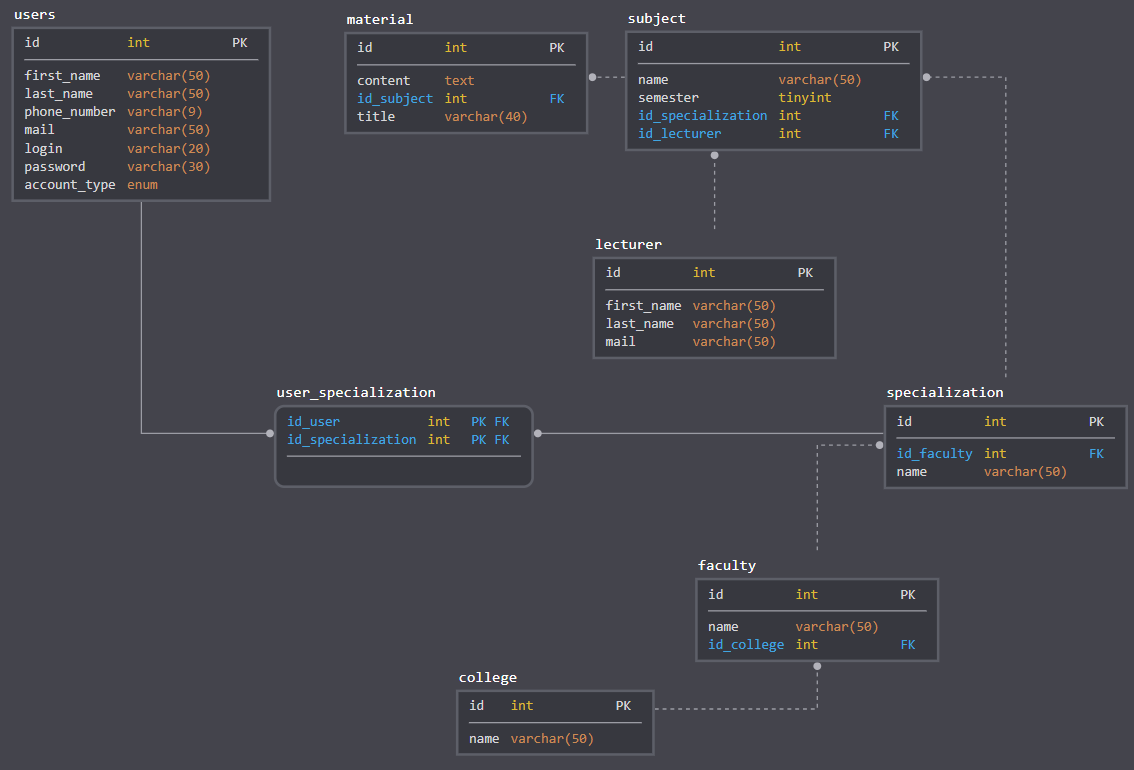
\includegraphics[width=1\linewidth]{relation_model}
			\end{figure}
		\subsection{MySQL}
			\subsubsection{Zapytania dotyczące 'Colleges'}
			\begin{lstlisting}
SP_GET_ALL = "SELECT  `Id`, `Name` FROM colleges";
SP_GET_FILTER = "SELECT  `Id`, `Name` FROM colleges {0}";
SP_GET_BYPAGE = "SELECT * FROM colleges {1} ORDER BY {0} LIMIT {2}, {3}; SELECT COUNT(*) FROM colleges {1};";
SP_GET_BYID = "SELECT  `Id`, `Name` FROM colleges WHERE Id = @ref_id";
SP_ADD = "INSERT INTO colleges ( Id, Name) VALUES ( @Id, @Name) ";
SP_ADD1 = "INSERT INTO colleges ( Id, Name) VALUES ( @Id, @Name) SELECT @Id = @@IDENTITY";
SP_UPDATE = "UPDATE colleges SET Name = @Name WHERE Id = @Id";
SP_DELETE = "DELETE FROM colleges WHERE Id=@ref_id";
SP_DELETE_FILTER = "DELETE FROM colleges {0}";
SP_GET_LOOKUP = "SELECT Id, Name FROM colleges";			
			\end{lstlisting}
			\subsubsection{Zapytania dotyczące 'Faculties'}
			\begin{lstlisting}
SP_GET_ALL = "SELECT  `Id`, `Name`, `College_Id` FROM faculties";
SP_GET_FILTER = "SELECT  `Id`, `Name`, `College_Id` FROM faculties {0}";
SP_GET_BYPAGE = "SELECT * FROM faculties {1} ORDER BY {0} LIMIT {2}, {3}; SELECT COUNT(*) FROM faculties {1};";
SP_GET_BYID = "SELECT  `Id`, `Name`, `College_Id` FROM faculties WHERE Id = @ref_id";
SP_ADD = "INSERT INTO faculties ( Id, Name, College_Id) VALUES ( @Id, @Name, @College_Id) ";
SP_ADD1 = "INSERT INTO faculties ( Id, Name, College_Id) VALUES ( @Id, @Name, @College_Id) SELECT @Id = @@IDENTITY";
SP_UPDATE = "UPDATE faculties SET Name = @Name, College_Id = @College_Id WHERE Id = @Id";
SP_DELETE = "DELETE FROM faculties WHERE Id=@ref_id";
SP_DELETE_FILTER = "DELETE FROM faculties {0}";
SP_GET_LOOKUP = "SELECT Id, Name FROM faculties";
			
			\end{lstlisting}
\clearpage	\subsubsection{Zapytania dotyczące 'Lecturers'}
			\begin{lstlisting}
SP_GET_ALL = "SELECT  `Id`, `Name`, `Surname`, `EmailAddress` FROM lecturers";
SP_GET_FILTER = "SELECT  `Id`, `Name`, `Surname`, `EmailAddress` FROM lecturers {0}";
SP_GET_BYPAGE = "SELECT * FROM lecturers {1} ORDER BY {0} LIMIT {2}, {3}; SELECT COUNT(*) FROM lecturers {1};";
SP_GET_BYID = "SELECT  `Id`, `Name`, `Surname`, `EmailAddress` FROM lecturers WHERE Id = @ref_id";
SP_ADD = "INSERT INTO lecturers ( Id, Name, Surname, EmailAddress) VALUES ( @Id, @Name, @Surname, @EmailAddress) ";
SP_ADD1 = "INSERT INTO lecturers ( Id, Name, Surname, EmailAddress) VALUES ( @Id, @Name, @Surname, @EmailAddress) SELECT @Id = @@IDENTITY";
SP_UPDATE = "UPDATE lecturers SET Name = @Name, Surname = @Surname, EmailAddress = @EmailAddress WHERE Id = @Id";
SP_DELETE = "DELETE FROM lecturers WHERE Id=@ref_id";
SP_DELETE_FILTER = "DELETE FROM lecturers {0}";
SP_GET_LOOKUP = "SELECT Id, Name FROM lecturers";
			
			\end{lstlisting}
			\subsubsection{Zapytania dotyczące 'Materials'}
			\begin{lstlisting}
SP_GET_ALL = "SELECT  `Id`, `Title`, `Content`, `Subject_Id` FROM materials";
SP_GET_FILTER = "SELECT  `Id`, `Title`, `Content`, `Subject_Id` FROM materials {0}";
SP_GET_BYPAGE = "SELECT * FROM materials {1} ORDER BY {0} LIMIT {2}, {3}; SELECT COUNT(*) FROM materials {1};";
SP_GET_BYID = "SELECT  `Id`, `Title`, `Content`, `Subject_Id` FROM materials WHERE Id = @ref_id";
SP_ADD = "INSERT INTO materials ( Id, Title, Content, Subject_Id) VALUES ( @Id, @Content, @Subject_Id) ";
SP_ADD1 = "INSERT INTO materials ( Id,Title, Content, Subject_Id) VALUES ( @Id, @Content, @Subject_Id) SELECT @Id = @@IDENTITY";
SP_UPDATE = "UPDATE materials SET Title = @Title, Content = @Content, Subject_Id = @Subject_Id WHERE Id = @Id";
SP_DELETE = "DELETE FROM materials WHERE Id=@ref_id";
SP_DELETE_FILTER = "DELETE FROM materials {0}";
SP_GET_LOOKUP = "SELECT Id, Title, Content FROM materials";
			
			\end{lstlisting}
\clearpage	\subsubsection{Zapytania dotyczące 'Specializations'}
			\begin{lstlisting}
SP_GET_ALL = "SELECT  `Id`, `Name`, `Faculty_Id` FROM specializations";
SP_GET_FILTER = "SELECT  `Id`, `Name`, `Faculty_Id` FROM specializations {0}";
SP_GET_BYPAGE = "SELECT * FROM specializations {1} ORDER BY {0} LIMIT {2}, {3}; SELECT COUNT(*) FROM specializations {1};";
SP_GET_BYID = "SELECT  `Id`, `Name`, `Faculty_Id` FROM specializations WHERE Id = @ref_id";
SP_ADD = "INSERT INTO specializations ( Id, Name, Faculty_Id) VALUES ( @Id, @Name, @Faculty_Id) ";
SP_ADD1 = "INSERT INTO specializations ( Id, Name, Faculty_Id) VALUES ( @Id, @Name, @Faculty_Id) SELECT @Id = @@IDENTITY";
SP_UPDATE = "UPDATE specializations SET Name = @Name, Faculty_Id = @Faculty_Id WHERE Id = @Id";
SP_DELETE = "DELETE FROM specializations WHERE Id=@ref_id";
SP_DELETE_FILTER = "DELETE FROM specializations {0}";
SP_GET_LOOKUP = "SELECT Id, Name FROM specializations";
			
			\end{lstlisting}
 			\subsubsection{Zapytania dotyczące 'Subjects'}
			\begin{lstlisting}
SP_GET_ALL = "SELECT  `Id`, `Name`, `Semester`, `Lecturer_Id`, `Specialization_Id` FROM subjects";
SP_GET_FILTER = "SELECT  `Id`, `Name`, `Semester`, `Lecturer_Id`, `Specialization_Id` FROM subjects {0}";
SP_GET_BYPAGE = "SELECT * FROM subjects {1} ORDER BY {0} LIMIT {2}, {3}; SELECT COUNT(*) FROM subjects {1};";
SP_GET_BYID = "SELECT  `Id`, `Name`, `Semester`, `Lecturer_Id`, `Specialization_Id` FROM subjects WHERE Id = @ref_id";
SP_ADD = "INSERT INTO subjects ( Id, Name, Semester, Lecturer_Id, Specialization_Id) VALUES ( @Id, @Name, @Semester, @Lecturer_Id, @Specialization_Id) ";
SP_ADD1 = "INSERT INTO subjects ( Id, Name, Semester, Lecturer_Id, Specialization_Id) VALUES ( @Id, @Name, @Semester, @Lecturer_Id, @Specialization_Id) SELECT @Id = @@IDENTITY";
SP_UPDATE = "UPDATE subjects SET Name = @Name, Semester = @Semester, Lecturer_Id = @Lecturer_Id, Specialization_Id = @Specialization_Id WHERE Id = @Id";
SP_DELETE = "DELETE FROM subjects WHERE Id=@ref_id";
SP_DELETE_FILTER = "DELETE FROM subjects {0}";
SP_GET_LOOKUP = "SELECT Id, Name FROM subjects";
			
			\end{lstlisting}
\clearpage	\subsubsection{Zapytania dotyczące 'Users'}
			\begin{lstlisting}
SP_GET_ALL = "SELECT  `Id`, `FirstName`, `LastName`, `PhoneNumber`, `MailAddress`, `Login`, `Password`, `AccountType` FROM users";
SP_GET_FILTER = "SELECT  `Id`, `FirstName`, `LastName`, `PhoneNumber`, `MailAddress`, `Login`, `Password`, `AccountType` FROM users {0}";
SP_GET_BYPAGE = "SELECT * FROM users {1} ORDER BY {0} LIMIT {2}, {3}; SELECT COUNT(*) FROM users {1};";
SP_GET_BYID = "SELECT  `Id`, `FirstName`, `LastName`, `PhoneNumber`, `MailAddress`, `Login`, `Password`, `AccountType` FROM users WHERE Id = @ref_id";
SP_ADD = "INSERT INTO users ( Id, FirstName, LastName, PhoneNumber, MailAddress, Login, Password, AccountType) VALUES ( @Id, @FirstName, @LastName, @PhoneNumber, @MailAddress, @Login, @Password, @AccountType) ";
SP_ADD1 = "INSERT INTO users ( Id, FirstName, LastName, PhoneNumber, MailAddress, Login, Password, AccountType) VALUES ( @Id, @FirstName, @LastName, @PhoneNumber, @MailAddress, @Login, @Password, @AccountType) SELECT @Id = @@IDENTITY";
SP_UPDATE = "UPDATE users SET FirstName = @FirstName, LastName = @LastName, PhoneNumber = @PhoneNumber, MailAddress = @MailAddress, Login = @Login, Password = @Password, AccountType = @AccountType WHERE Id = @Id";
SP_DELETE = "DELETE FROM users WHERE Id=@ref_id";
SP_DELETE_FILTER = "DELETE FROM users {0}";
SP_GET_LOOKUP = "SELECT Id, FirstName FROM users";
			
			\end{lstlisting}
			\subsubsection{Zapytania dotyczące 'UserSpecializations'}
			\begin{lstlisting}
SP_GET_ALL = "SELECT  `User_Id`, `Specialization_Id` FROM userspecializations";
SP_GET_FILTER = "SELECT  `User_Id`, `Specialization_Id` FROM userspecializations {0}";
SP_GET_BYPAGE = "SELECT * FROM userspecializations {1} ORDER BY {0} LIMIT {2}, {3}; SELECT COUNT(*) FROM userspecializations {1};";
SP_GET_BYID = "SELECT  `User_Id`, `Specialization_Id` FROM userspecializations WHERE User_Id = @ref_id";
SP_ADD = "INSERT INTO userspecializations ( User_Id, Specialization_Id) VALUES ( @User_Id, @Specialization_Id) ";
SP_ADD1 = "INSERT INTO userspecializations ( User_Id, Specialization_Id) VALUES ( @User_Id, @Specialization_Id) SELECT @User_Id = @@IDENTITY";
SP_UPDATE = "UPDATE userspecializations SET Specialization_Id = @Specialization_Id WHERE User_Id = @User_Id";
SP_DELETE = "DELETE FROM userspecializations WHERE User_Id=@ref_id";
SP_DELETE_FILTER = "DELETE FROM userspecializations {0}";
SP_GET_LOOKUP = "SELECT User_Id, User_Id FROM userspecializations";
			
			\end{lstlisting}
		\subsection{Środowisko}
			Baza danych znajduje się w chmurze Heroku. Łączymy się z nią za pomocą...
	\section{Testy}
		Baza działa... Jakieś info z Heroku można tutaj dać.
\end{document}